\chapter{Software und Hardware}

Folgendes Kapitel umfasst grundlegende Hardwareanforderungen, die verwendete Software und vorbereitende Arbeiten zur Verwendung des Kamerasystems und zum Einlernen benutzerdefinierter Objekte.

\section{Konfiguration des Kamerasystems}

Für die Bearbeitung wurde ursprünglich eine Microsoft Kinect V2 Kamera verwendet. Aufgrund von Hardwarekompatibilitäts- und Treiberproblemen zwischen Kinect und aktueller Hardware und dem schlechten \ac{ROS}-Treibersupport der Kinect für den Anwendungsfall, wurde im späteren Verlauf eine Intel Realsense 435 verwendet. Diese bietet zudem die Möglichkeit einer Befestigung an der Roboterhand. Weitere Tests wurden somit ausschließlich mit der RealSense durchgeführt.

\subsection{Technische Daten}

Folgender Abschnitt behandelt die technischen Daten der Microsoft Kinect V2 und der Intel RealSense 435.

\paragraph{Microsoft Kinect}

Bei der Microsoft Kinect handelt es sich um ein ursprünglich für die Spielkonsole \textit{Xbox} entwickeltes Kamerasystem, das mit einer RGB- und Infrarotkamera zur Tiefenmessung ausgestattet ist. Die RGB-Kamera löst mit $1920 \cdot 1080$ Pixeln auf, die Infrarotkamera mit $512 \cdot 424$. Beide Kameras besitzen eine maximale Bildwiederholrate von 30 Bildern pro Sekunde \cite{sung_real-time_2019}.

\begin{figure}[ht]
    \centering
    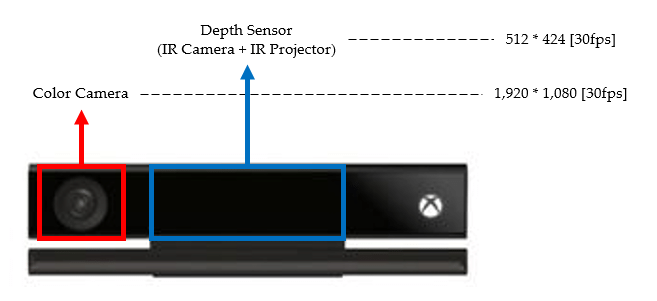
\includegraphics[width=\textwidth]{Bilder/kinect_aufbau.png}
    \caption{Aufbau der Microsoft Kinect v2 \cite[Abbildung~5]{sung_real-time_2019}}
    \label{fig:kinect_aufbau}
\end{figure}

Die Kinect wird aufgrund der vergleichsweise geringen Kosten und der Verfügbarkeit vieler Open-Source-Programme oft in der Forschung der Robotik eingesetzt. Da jedoch kaum Kompatibilität mit aktuellen Systemen vorhanden ist und kein direkter Nachfolger der Kinect V2 existiert, werden jedoch zunehmend andere Kamerasysteme wie die Intel RealSense eingesetzt.

Die minimale Distanz der Kinect V2 beträgt aufgrund der Sättigung des Sensors durch das reflektierte Infrarotlicht ungefähr $0,5m$ \cite[Kapitel~2.1]{noonan_repurposing_2015}. Die Abweichung nimmt mit steigender Entfernung zwischen Kamera und Bauteil leicht zu. Während ein hoher Offset von $-0,02m$ vorhanden ist, beträgt die Standardabweichung auch bei Entfernungen über $1m$ unter $0,002m$, was für den Anwendungsfall ausreichend genau ist \seeFig{fig:kinect_genauigkeit}.

\begin{figure}[ht]
    \centering
    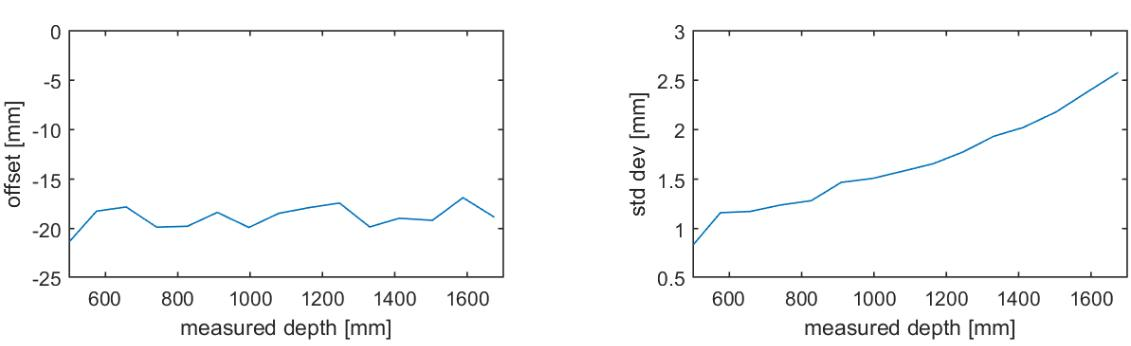
\includegraphics[width=\textwidth]{Bilder/kinect_genauigkeit.jpg}
    \caption{Genauigkeit der Microsoft Kinect v2 \cite[Abbildung~5]{chen_comparison_2017}}
    \label{fig:kinect_genauigkeit}
\end{figure}

Für die Verwendung der Kinect unter Linux-Systemen wird aufgrund der fehlenden offiziellen Herstellerunterstützung der inoffizielle \textit{libfreenect2} Treiber verwendet. Mit diesem können Informationen der RGB- und Infrarotkamera unter Linux ausgelesen werden \cite{xiang_libfreenect2_2016}.
Als Schnittstelle zwischen Kinect und \ac{ROS} Noetic wird das Paket \textit{iai\_kinect2} \cite{wiedemeyer_iai_2021} genutzt. Es stellt neben Funktionen zur Interaktion mit der Kinect über \textit{Topics} Werkzeuge zur Kalibrierung und Anzeige der Kamerabilder zur Verfügung.

\pagebreak
\paragraph{Intel Realsense} \label{subsec:intel_realsense}

Die Intel Realsense 435 hat im Vergleich zur Kinect V2 eine höhere Tiefenauflösung. Im Gegensatz zur Kinect wird hier nicht die \textit{\ac{ToF}}-Technik verwendet, sondern die Tiefe unter Verwendung einer Stereokamera berechnet \seeFig{fig:realsense_aufbau}. 

\begin{figure}[ht]
    \centering
    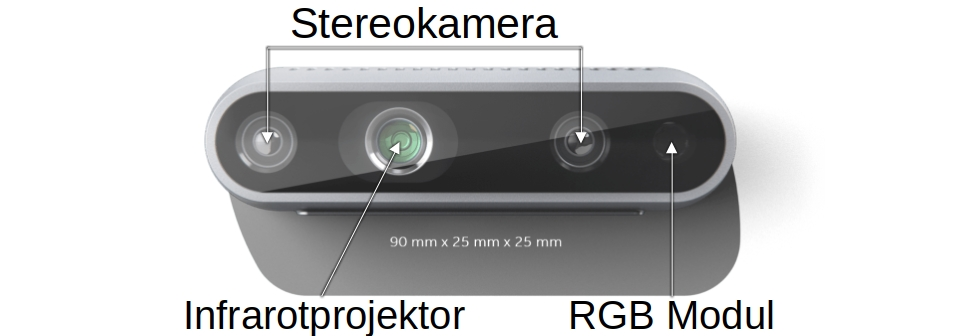
\includegraphics[width=9cm]{Bilder/realsense_aufbau.jpg}
    \caption{Aufbau der Intel RealSense 435, Abbildung nach \cite{intel_corporation_depth_2022}}
    \label{fig:realsense_aufbau}
\end{figure}

Um die Distanzdaten zu ermitteln, ist außerdem ein Infrarotlicht zur Beleuchtung des Aufnahmebereichs integriert, das die Genauigkeit mithilfe der Projektion von Beleuchtungsmustern erhöht \seeFig{fig:realsense_infrarot}. Durch die geringe Baugröße von $90mm \cdot 25mm \cdot 25mm$ und die Kombination Strom- und Datenfluss in einem Kabel kann die RealSense mit geringem Aufwand am Handstück des Roboterarms befestigt werden. Die für Stereokameras typische ungenauere Tiefenmessung im Vergleich zu \ac{ToF}-Systemen wird durch den Infrarotprojektor kompensiert, weshalb die Kamera für diese Anwendung geeignet ist. 

\begin{figure}[ht]
    \centering
    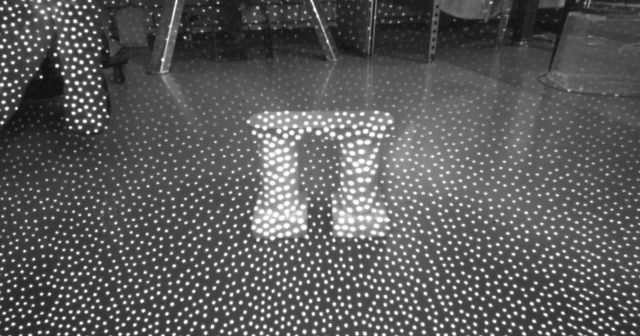
\includegraphics[width=7.12cm]{Bilder/realsense_infrarot.jpg}
    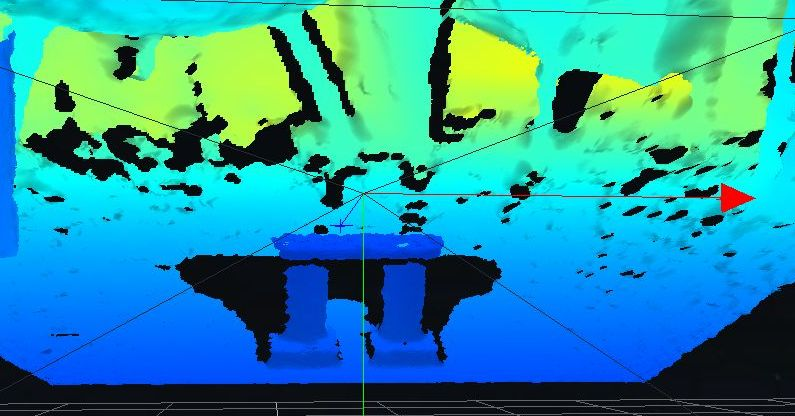
\includegraphics[width=7.14cm]{Bilder/realsense_3d.jpg}
    \caption{Infrarotproj. und 3D-Bild der Intel RealSense 435}
    \label{fig:realsense_infrarot}
\end{figure}

Zur Ermittlung der Genauigkeit wurden Präzisionstests für die Distanz zwischen Kamera und Bauteil durchgeführt. Die Messungen wurden in einem Distanzbereich zwischen $0,3 m$ und $1,0 m$ getätigt, da die minimal mögliche Distanz der RealSense zur Tiefenmessung $0,28 m$ beträgt. Diese Distanz ist auf die Funktionsweise der Stereokamera-Technik zurückzuführen. \refFig{fig:realsense_genauigkeit} zeigt die prozentuale mittlere Abweichung des gemessenen Abstandes zwischen Kamera- und Bauteiloberfläche in Bezug auf den realen Abstand. Dabei überschreitet die Abweichung in keinem Fall $-2 \%$. Bei einem Offset der Messwerte von $+0,001m$ beträgt die maximale Abweichung $\pm1 \%$. Bei geringen Entfernungen ist sie durchschnittlich kleiner. Die im Versuch gemessene Abweichung mit einem Wert von maximal $2\%$ stimmt mit der von Intel angegebenen Genauigkeit überein \cite{intel_corporation_depth_2022}.

\begin{figure}[ht]
    \centering
    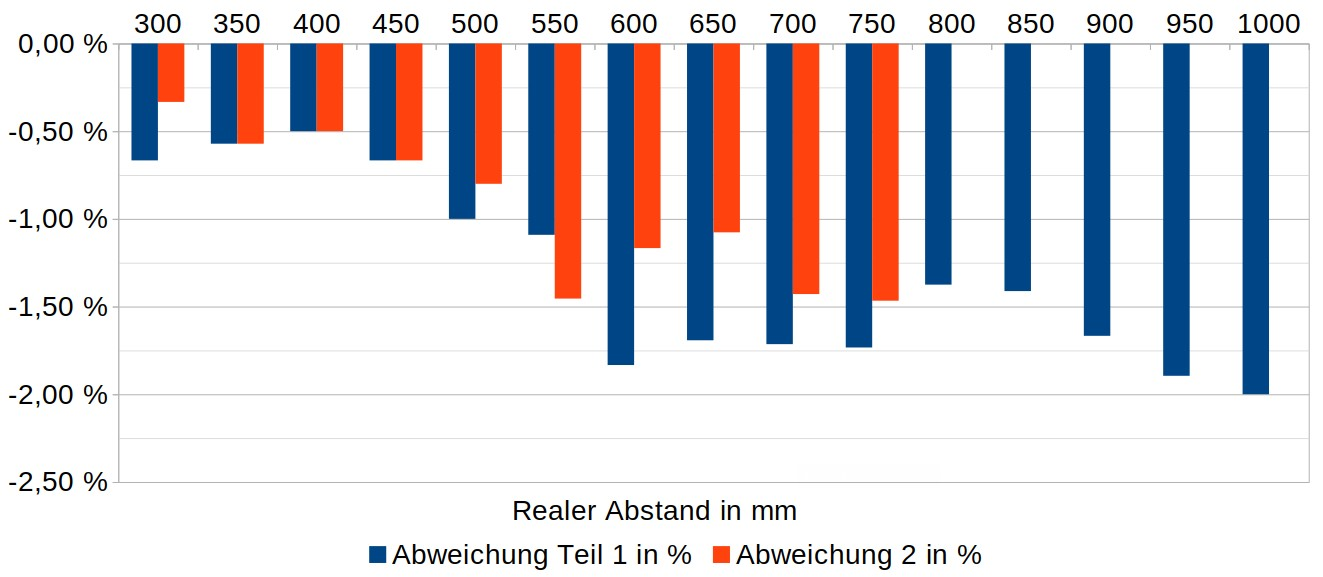
\includegraphics[width=\textwidth]{Bilder/realsense_genauigkeit.jpg}
    \caption{Genauigkeit der Intel RealSense 435}
    \label{fig:realsense_genauigkeit}
\end{figure}

Die Genauigkeit auf planarer Ebene variiert mit Änderung der Entfernung, verschiedenen Bildauflösungen, Version des verwendeten Algorithmus und dem für den Einlernprozess verwendeten Datensatz. Aufgrund der dadurch entstehenden hohen Variabilität sind Tests dieser im Rahmen der Arbeit nicht zielführend. Bei allen durchgeführten Tests war die Erkennung jedoch für den Anwendungsfall mit einer Abweichung von wenigen Millimetern ausreichend genau.

Intel stellt für die Verwendung der RealSense unter Linux das \textit{LibRealSense open source \ac{SDK}} \cite{intel_corporation_intelrealsenselibrealsense_2022} bereit. Mit diesem können, ähnlich wie beim Treiber der Kinect, Daten der RGB-Kamera ausgelesen werden. Die 3D-Daten werden in diesem Fall über eine Kombination der Bilddaten beider Kameras berechnet und nicht wie bei \textit{\ac{ToF}} direkt gemessen. Der Treiber stellt \textit{Point Clouds} - wobei es sich um dreidimensionale, aus einzelnen Punkten zusammengesetzte Bilder handelt - mit optionaler Überlagerung der Farbinformationen zur Verfügung.

Die Integration in das \ac{ROS} erfolgt mit dem offiziellen \textit{realsense-ros} \textit{Package} \cite{intel_corporation_ros_2022}. Dieses stellt die notwendigen \textit{Topics} für die Verwendung des Bilderkennungsalgorithmus und der Abstandsmessung bereit. Dazu zählt neben dem RGB-Bild und den Hardwareinformationen die Integration der \textit{Point Cloud}, mit der der Abstand zwischen Objekt und Kamerasystem bestimmt werden kann \seeFig{fig:realsense_rviz}. Zum Starten des in \textit{realsense-ros} enthaltenen \textit{realsense2\_camera}-Pakets wird eine Konfiguration verwendet, die zum Erreichen einer höheren Kompatibilität mit anderen \ac{ROS}-Paketen die \textit{Point Cloud} nach dem \textit{OpenNI}-Standard bereitstellt \seeAtt{sec:realsense}. Dabei handelt es sich um einen weit verbreiteten, offiziell eingestellten aber weiterentwickelten, Standard zur Verbesserung der Interoperabilität zwischen Software und Hardware \cite{occipital_openni_2022}.

\begin{figure}[ht]
    \centering
    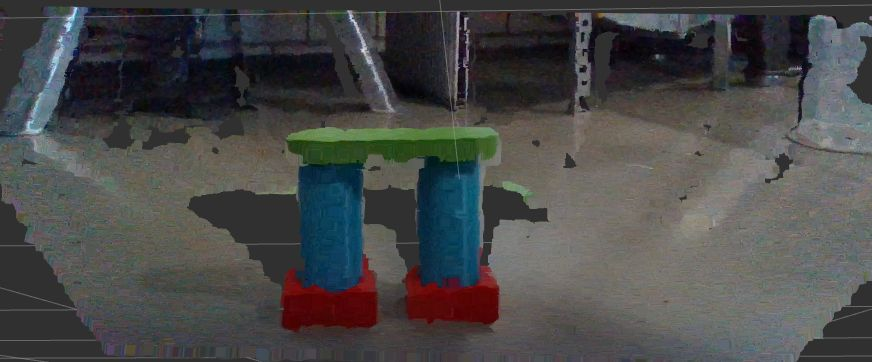
\includegraphics[width=\textwidth]{Bilder/realsense_rviz.jpg}
    \caption{RealSense Point Cloud in Rviz}
    \label{fig:realsense_rviz}
\end{figure}

\subsection{Kalibrierung}

Für die Positionserkennung muss eine Transformation zwischen Roboter- und Kamerakoordinatensystem durchgeführt werden. Diese kann mithilfe einer Hand-Auge-Kalibrierung berechnet werden. Außerdem ist ein Abgleich der Koordinaten zwischen RGB- und Tiefensensor möglich, da durch Ungenauigkeiten bei der Kameraausrichtung und Bildverzerrung Koordinaten in $x$-$y$-Ebene abweichen können. 

\subsubsection{RGB-D Kalibrierung} 

Zum Abgleich zwischen RGB- und Tiefenkamera kann eine RGB-D Kalibrierung durchgeführt werden. 

\paragraph{Microsoft Kinect}

Für die Durchführung mit einer Kinect V2 kann beispielsweise das im Paket \textit{iai\_kinect2} enthaltene Programm zur Kalibrierung genutzt werden \cite{wiedemeyer_iai_2021}. Diese gleicht Abweichungen durch Verzerrung, Rotation und Verschiebung zwischen den Kamerasystemen aus \cite[Beispieldaten]{wiedemeyer_iai_kinect2kinect2_bridgedata_2015}.

Die Kalibrierung erfolgt in diesem Fall mithilfe eines Schachbrett-Musters. Dieses kann bei bekannten Kameraparametern der 2D-RGB-Kamera zur dreidimensionalen Positionsbestimmung eines Objekts im Raum genutzt werden \cite{opencvorg_camera_2019}. Somit ist eine Berechnung der Abweichung zwischen den von den 2D- und 3D-Kameras erkannten Parametern möglich.

\pagebreak
Um die Kalibrierung durchzuführen, wird die Kinect nacheinander in mehreren Positionen relativ zum Kalibrierungsmuster aufgestellt. Nach jeder Bewegung des Musters wird ein Bild mit beiden Kameras der Kinect gemacht, was zum Abgleich genutzt werden kann. Es wird in der Dokumentation von \textit{iai\_kinect2} empfohlen, den Abstand und die Neigung des Kalibrierungsmusters zu verändern, um ein gutes Ergebnis zu erzielen \cite{wiedemeyer_iai_2021}.

\paragraph{Intel RealSense}

Die Intel RealSense ist im Gegensatz zur Kinect bei Verwendung des \textit{iai\_kinect2}-Treibers ab Werk kalibriert. Eine klassische manuelle Kalibrierung ohne spezielle Hardware führt laut Intel mit hoher Wahrscheinlichkeit zu einer Verschlechterung der Kalibrierung. Die aktuelle Firmware der RealSense bietet jedoch Optimierungsmöglichkeiten für diverse Parameter wie Ebenheit der \textit{Point Cloud} oder Distanzgenauigkeit. Diese sind hauptsächlich auf Abnutzungserscheinungen nach längerer Nutzung ausgelegt \cite{grunnet-jepsen_intel_2021}. Da es sich bei der verwendeten RealSense um ein neues Gerät mit ausreichender Genauigkeit handelt \seeFig{fig:realsense_genauigkeit}, wird auf eine Kalibrierung verzichtet.

\subsubsection{Hand-Auge-Kalibrierung}

Als Hand-Auge-Kalibrierung bezeichnet man die Ermittlung von homogenen Transformationsmatrizen zwischen dem Endeffektor des Roboters und dem Kamerasystem sowie die Transformation zwischen Welt- und Basiskoordinatensystem \cite[Kapitel~1]{tabb_solving_2017}.

Man unterscheidet hier zwischen zwei Fällen: Die Kamera kann entweder stationär nahe dem Roboter oder wie im vorliegenden Fall am Endeffektor befestigt werden. Letztere Möglichkeit hat den Vorteil, dass das Kamerasystem durch Anfahren des Bauteilmittelpunktes und mit einer geringen Entfernung zwischen Kamera und Objektoberfläche eine präzisere Steuerung erzielen kann.

Die Kalibrierung in \ac{ROS} kann mit dem \textit{moveit\_calibration}-Paket \cite{rauch_moveit_2022} durchgeführt werden. Dieses unterstützt beide erwähnten Konfigurationsmöglichkeiten. Die vom Programm durchgeführten Messungen erfolgen anhand eines visuellen Kalibriermusters mit distinktiven Formen, mit dem bei bekannter Größe die Lage des Kamerakoordinatensystems bestimmt werden kann. Dazu sollten zum Erfassen mindestens fünf Posen angefahren werden \cite{stechschulte_hand-eye_2022}.

Für den Anwendungsfall dieser Arbeit ist die manuelle Koordinatentransformation ausreichend, da die Lage des Kamerakoordinatensystems im Ursprung der RealSense nur in Relation zum Koordinatensystem, das vom Bewegungsplanungsprogramm von Steinbeck \cite{steinbeck_entwicklung_2022} verwendet wird, berechnet werden muss. Die Koordinatensysteme haben eine rotationsfreie Verschiebung. Die durchgeführte Transformation ist im \refSec{subsec:algorithmus_positionserkennung} näher beschrieben.

\subsection{Befestigung}

Die RealSense kann aufgrund der geringen Baugröße und niedriger Erschütterungsanfälligkeit in der Nähe des Endeffektors am Roboter befestigt werden. Datenübertragung und die Stromversorgung erfolgen über ein einziges USB-Kabel. Aufgrund des größeren Sichtfeldes und besserer Abdeckung des Arbeitsraumes wird die Kamera mit einer Drehung von $90$° gegenüber dem Endeffektor montiert (s. \refFig{fig:realsense_halter}, oben).

\begin{figure}[ht]
    \centering
    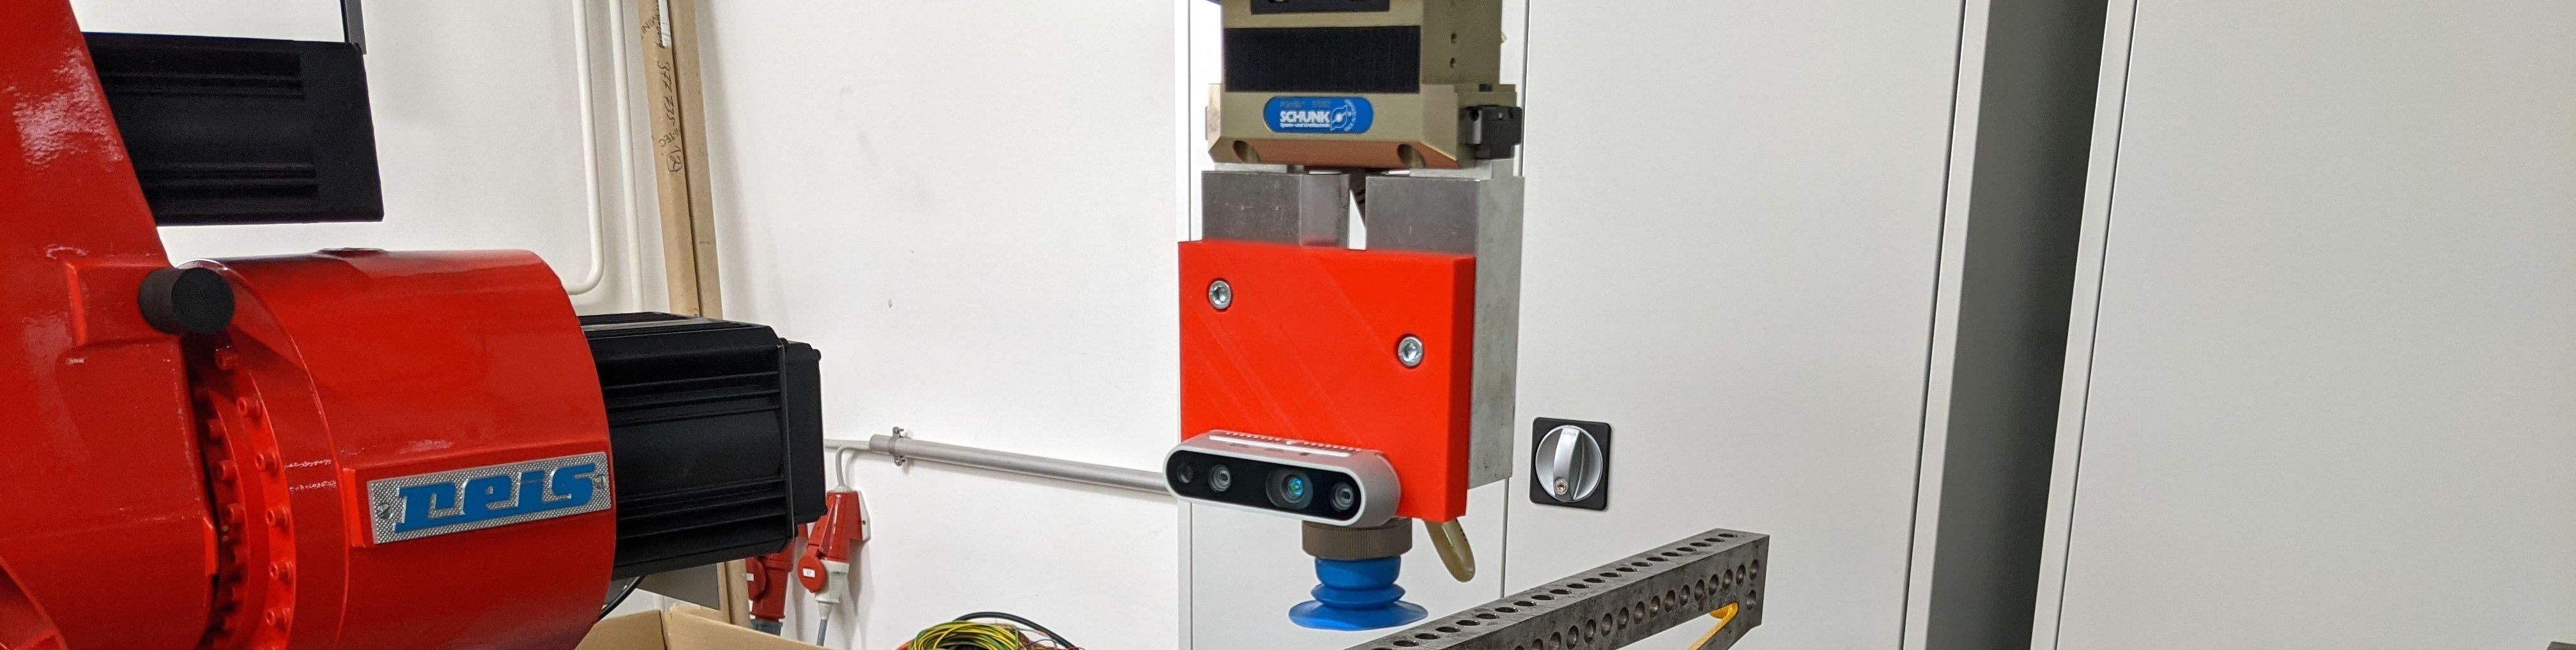
\includegraphics[width=\textwidth]{Bilder/realsense_halter.jpg}
    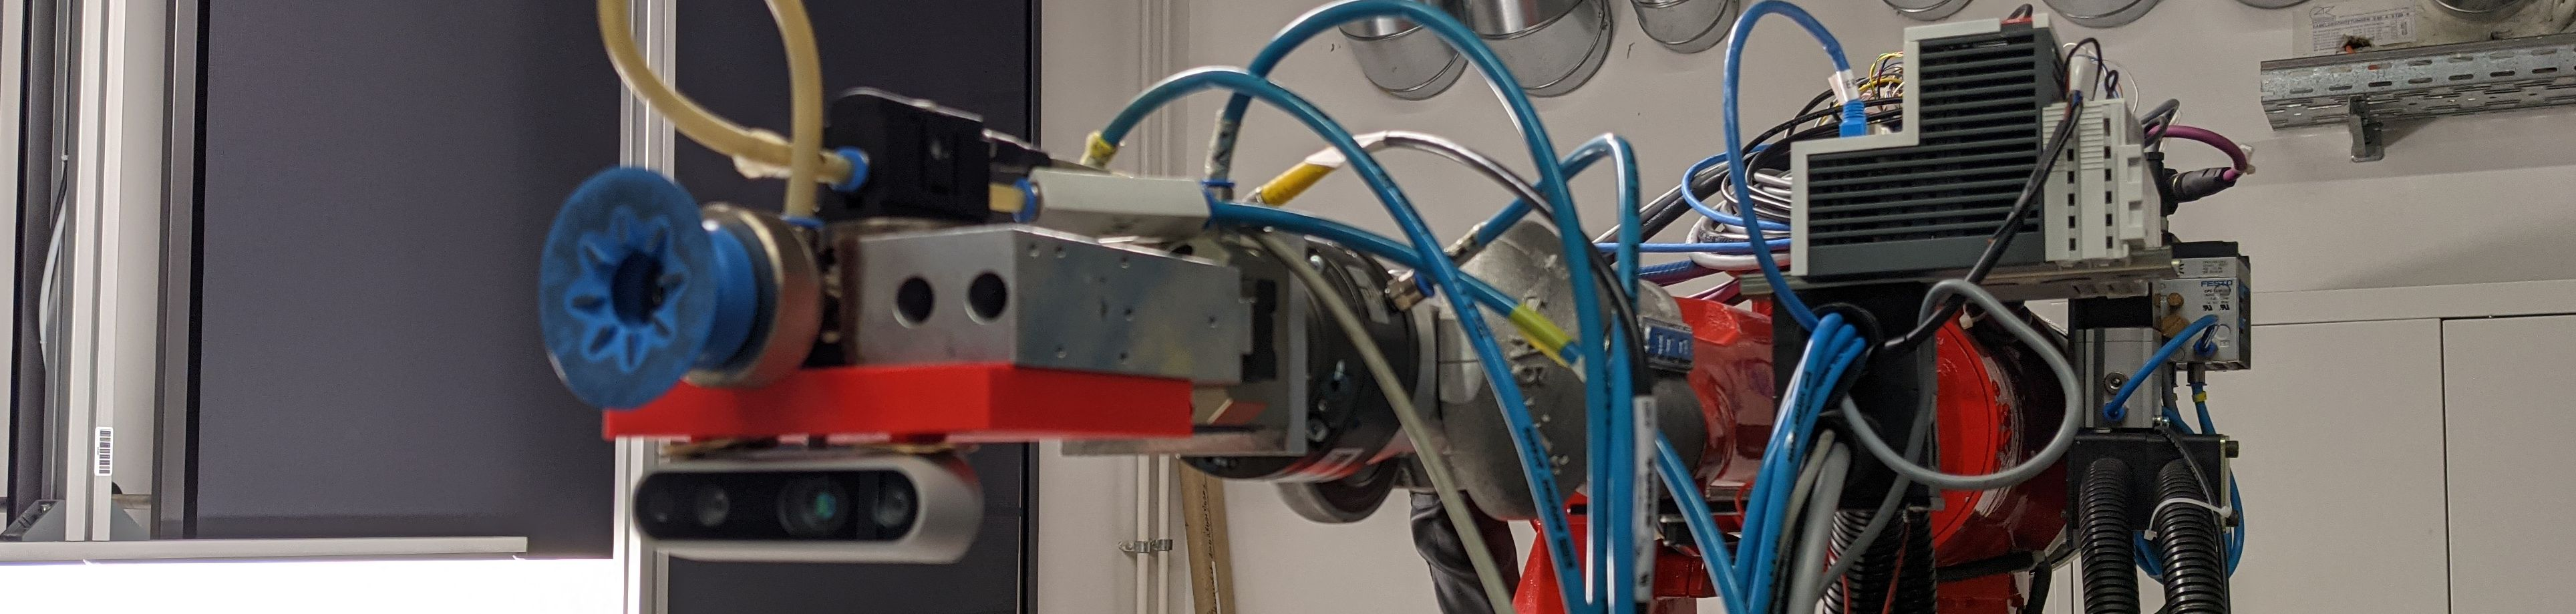
\includegraphics[width=\textwidth]{Bilder/realsense_halter2.jpg}
    \caption{Befestigung der Intel RealSense am Endeffektor}
    \label{fig:realsense_halter}
\end{figure}

\section{Implementierung der Objekterkennung}

\textit{\ac{YOLO}} eignet sich aufgrund schneller und ressourcenschonender Erkennung und Lokalisierung von Objekten ohne große Einschränkungen der Genauigkeit gut für den Anwendungsfall dieser Arbeit. Pro Zelle des Bildrasters können in \textit{YOLOv1} bis zu drei, in \textit{YOLOv3} bis zu neun Objekte gleichzeitig erkannt und lokalisiert werden \cite{bandyopadhyay_yolo_2021}. 

\subsection{Voraussetzungen für das Objekterkennungsprogramm}

Wegen der weitreichenden Kompatibilität und der langen Support-Dauer wird die Version \ac{ROS}-I verwendet. Verglichen mit dem verhältnismäßig neuen \ac{ROS}-II ist ein breiteres Spektrum an kompatibler Hardware und ausgereiften Paketen verfügbar. Bei Noetic handelt es sich um die aktuelle \textit{\ac{LTS}} Version des \ac{ROS}-I-Systems, die bis Mai 2025 unterstützt wird \cite[Abschnitt~3]{miura_distributions_2021}.

\begin{figure}[ht]
    \centering
    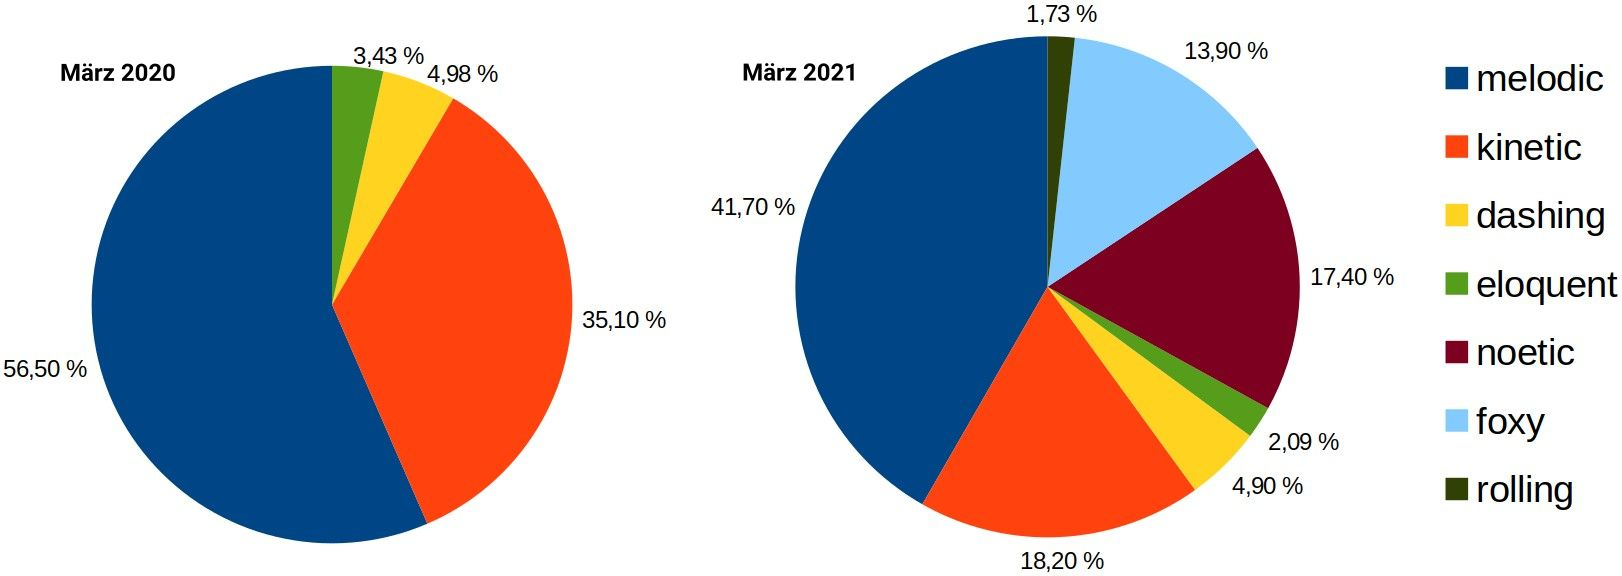
\includegraphics[width=\textwidth]{Bilder/ros_distro_usage.jpg}
    \caption{Anzahl der ROS-Downloads im März 2020 und 2021, Grafik nach \cite{scott_ros_2021}}
    \label{fig:ros_distro_usage}
\end{figure}

%\subsection{Systemanforderungen}

Für die Ausführung von \ac{ROS}-I Noetic wird ein Computer benötigt, der die Hardwareanforderungen von \textit{Ubuntu 20.04 LTS} erfüllt. Bei den Funktionstests wurde ein Computer mit \textit{x86-64}-Architektur verwendet, bei entsprechender Treiberunterstütung des Kamerasystems können aber auch \textit{ARM}-basierte Prozessoren genutzt werden. Für den Einlernprozess der Objekte \seeSec{subsec:add_objects} wird aufgrund der Notwendigkeit von \textit{Nvidia \ac{CUDA}} eine Grafikkarte des Herstellers \textit{Nvidia} benötigt. Zur Objekterkennung ist die Herstellerbindung nicht zwingend, aber für die Verwendung der Hardwarebeschleunigung notwendig. Die Erkennung über den Hauptprozessor des Computers ist somit grundsätzlich möglich, wird jedoch aufgrund der deutlich langsameren Verarbeitung der Objekte nicht empfohlen \cite{bjelonic_yolo_2016}.

%\subsection{Zusätzliche Kernprogramme}

Zur Nutzung des Programms und der Visualisierung werden zusätzlich zum \ac{ROS}-Hauptpaket das 3D-Visualisierungspaket \textit{RViz} \cite{ulisse_perusin_ros-visualizationrviz_2022} und das Bewegungs-planungs-Framework \textit{Moveit} \cite{ioan_a_sucan_moveit_nodate} benötigt. Nähere Informationen zu \textit{MoveIt} sind in der Arbeit von Steinbeck aufgeführt \cite[Abschnitt~3.2]{steinbeck_entwicklung_2022}.


Für die Aufnahme der Objekte müssen deren Art und Position bekannt sein. Durch die Kombination der zwei- und dreidimensionalen Bilddaten kann die Erkennung verschiedener Objekte mithilfe des RGB-Bildes erfolgen. Nach Berechnung des Mittelpunktes der \textit{Bounding Boxes} kann der Abstand zwischen Kamerasystem und der Objektoberfläche mithilfe des 3D-Bildes bestimmt werden. Somit sind alle Koordinaten der vom Greifer anzufahrenden Position bekannt.

\subsection{Training des YOLO-Algorithmus} \label{subsec:add_objects}

Zur Erkennung der in der Arbeit verwendeten Objekte müssen diese durch einen Einlernprozess als sogenannte \textit{Weights} gespeichert werden. Von jedem Objekt werden dazu zuerst mehrere Bilder mit verschiedenen Orientierungen, Lichtverhältnissen und in unterschiedlichen Umgebungen gemacht. Die Genauigkeit steigt üblicherweise mit der Anzahl der Bilder und den Iterationen im Einlernprozess. Diese Bilder müssen anschließend mit \textit{Bounding Boxes} und Objektnamen versehen werden. Die Bounding Boxes werden hier mit dem Programm \textit{LabelImg} \cite{tzutalin_labelimg_2015} erstellt, das das \textit{\ac{YOLO}} Format nativ unterstützt. Sie werden so genau wie möglich auf das Objekt angepasst, sodass die äußeren Punkte die Kanten des Rechtecks berühren. So ist eine möglichst genaue Positionserkennung im späteren Verlauf möglich. Der Datensatz ist unabhängig von der verwendeten \textit{\ac{YOLO}}-Version anwendbar. \refFig{fig:labelimg} zeigt beispielhaft den Aufbau einer Textdatei zur Beschreibung des Labels. Für das Training des neuronalen Netzes wird für jedes Bild eine solche Datei benötigt. Diese setzt sich aus einer Nummer für die Klasse des Objekts, dem Mittelpunkt der \textit{Bounding Box} und der Breite und Höhe dieser zusammen. Die Nummer der Objektklasse richtet sich hier nach der Reihenfolge in einer weiteren Textdatei, die die Klassennamen enthält. Pro Bild können auch mehrere, durch Zeilenumbrüche getrennte, \textit{Bounding Boxes} definiert werden.

\begin{figure}[ht]
    \centering
    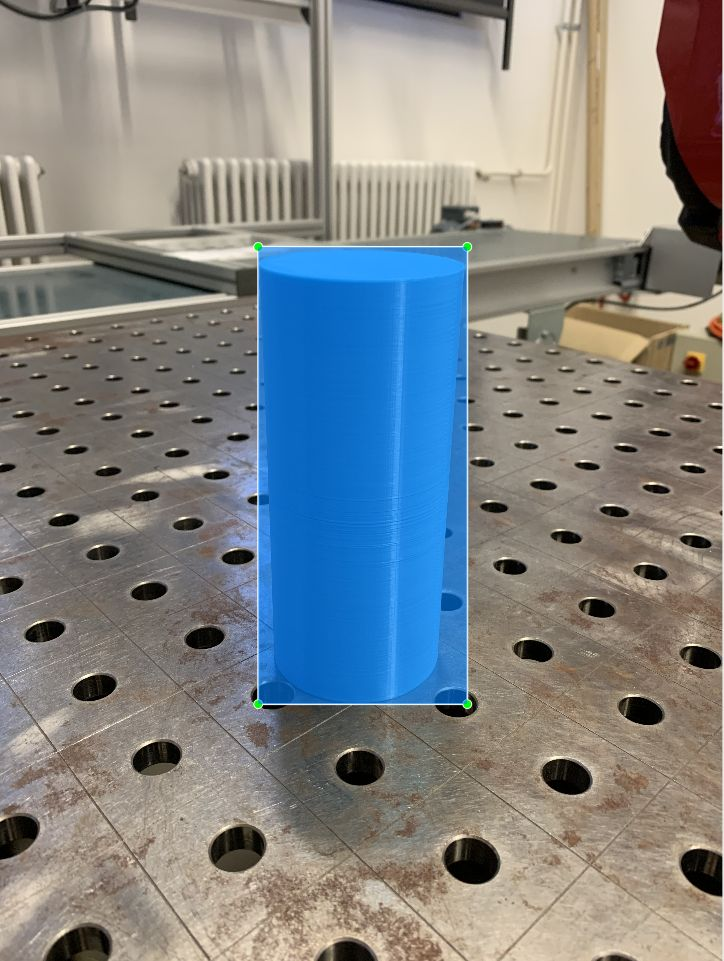
\includegraphics[width=4cm]{Bilder/labelimg.jpg}
    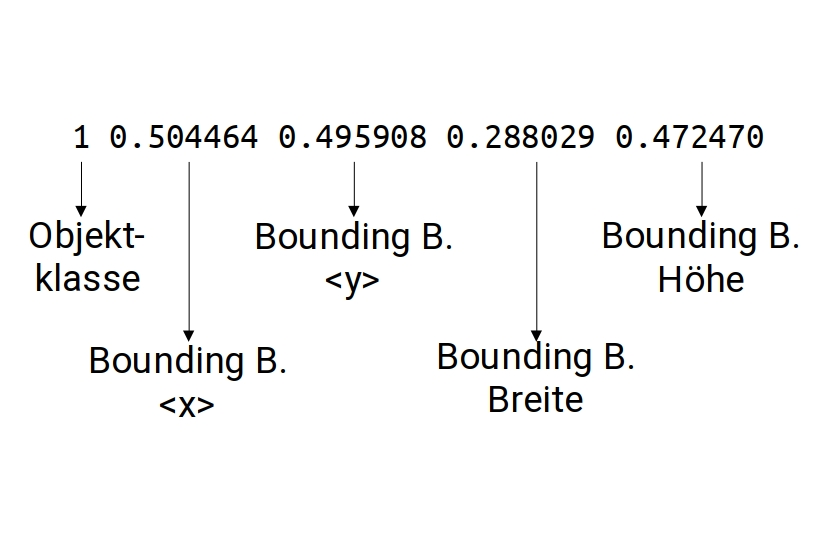
\includegraphics[width=10cm]{Bilder/boundingbox_struktur.jpg}
    \caption{YOLO Label}
    \label{fig:labelimg}
\end{figure}

Das \textit{Darknet} Framework beinhaltet Tools zum Training mit dem durch beispielsweise \textit{LabelImg} erstellten Datensatz. Dieser besteht aus Bildern, in denen ein oder mehrere zu erkennende Objekte enthalten sind und den erwähnten Textdateien mit Informationen über die \textit{Bounding Box}-Positionen. Das Training muss mit der gleichen Version des Algorithmus erfolgen, die später zur Erkennung genutzt wird.

Für das Training des verwendeten \textit{YOLOv3 Tiny}-Algorithmus wurde die in \refAtt{sec:darknet} aufgeführte Konfiguration mit einem Datensatz aus ungefähr 300 Bildern pro Objekt genutzt. Die generierten \textit{Weights} können an die entsprechende Stelle des \textit{rv6l\_3d}-Programms kopiert werden, um eine Objekterkennung zu ermöglichen. Der Einlernprozess wurde nach $10000$ Iterationen gestoppt, da die Genauigkeit bei den verwendeten Objekten mit mehr Wiederholungen nur wenig erhöht wird \seeFig{fig:darknet_iterationen}.

\begin{figure}[ht]
    \centering
    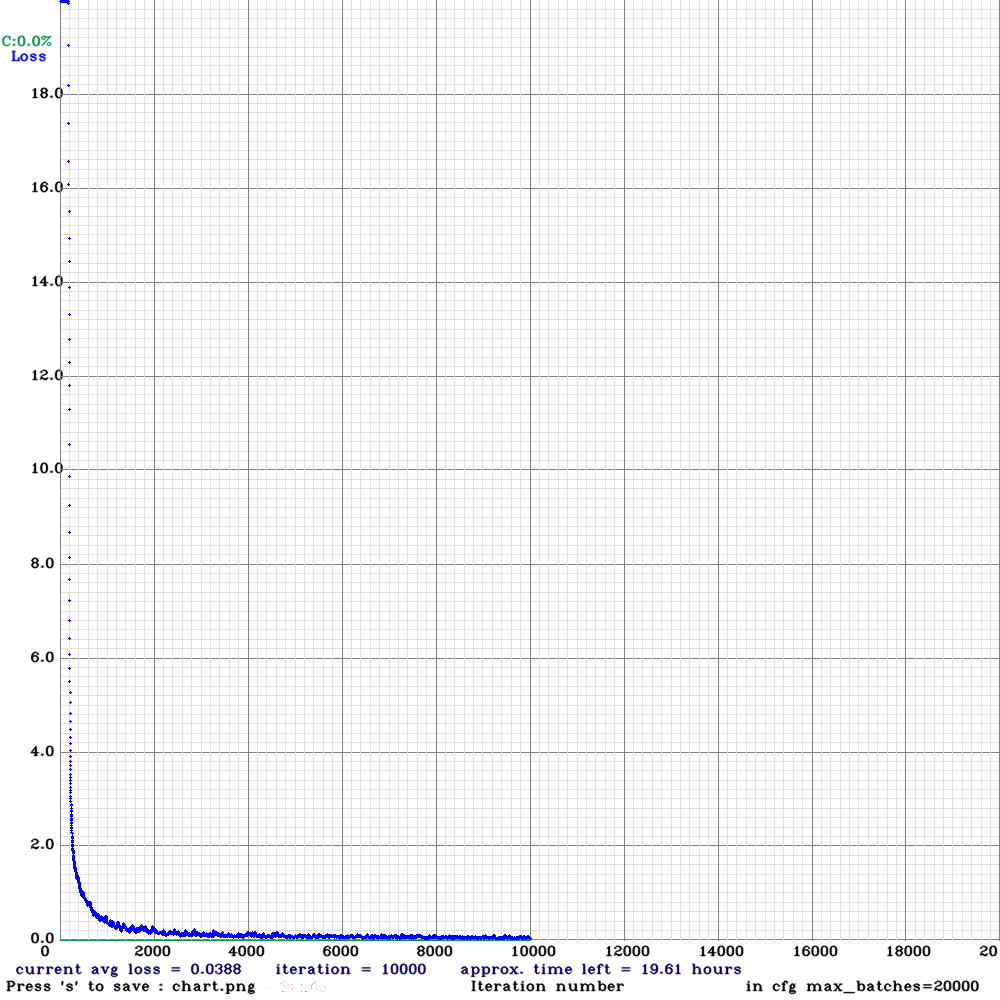
\includegraphics[width=\textwidth]{Bilder/darknet_iterationen.png}
    \caption{Darknet Iterationen [generiert mit Darknet]}
    \label{fig:darknet_iterationen}
\end{figure}

\pagebreak
\subsection{rv6l\_3d-Paket} \label{subsec:rv6l_3d}

Die Grundlage für die Positionserkennung mit \textit{Darknet} in \ac{ROS} bildet das \textit{rv6l\_3d}-Paket \seeAtt{sec:rv6l_3d}. Dabei handelt es sich um ein für diese Anwendung erstelltes Paket für \ac{ROS}, das auf dem 2016 von IntelligentRoboticsLabs veröffentlichten \textit{darknet\_ros\_3d} \cite{intelligentroboticslabs_darknet_ros_3d_2021} basiert. Dieses baut wiederum auf \textit{darknet\_ros} \cite{bjelonic_yolo_2016} auf. Eine Übersicht der Zusammenhänge zwischen den Paketen ist in \refSec{sec:programmstruktur} zu finden. Modifikationen umfassen die Entfernung nicht benötigter Funktionen, eine Mittelpunktberechnung der \textit{Bounding Boxes} und Anpassungen auf das Programm zur Handhabung der Bauteile. Die Kernfunktionalität des \textit{rv6l\_3d}-Pakets besteht in der Bereitstellung dreidimensionaler Objektmittelpunktkoordinaten unter Verwendung einer 3D-Kamera. Das Projekt nutzt die von \textit{darknet\_ros} zur Verfügung gestellten Daten zur Erkennung der planaren Objektposition und gleicht diese mit dem von einer Tiefenkamera gemessenen oder Stereokamera berechneten dreidimensionalen Bild ab, um den Abstand zwischen Kamera und Bauteiloberfläche zu ermitteln.

Die wichtigsten Modifikationen des Pakets umfassen das Entfernen der Marker, die zur Visualisierung der \textit{Bounding Boxes} in \textit{Rviz} dienen, die Berechnung der Objektmittelpunkte sowie Anpassungen des \textit{Topics} mit den Objektpositionen. Somit werden statt vollständigen \textit{Bounding Boxes} die Koordinaten der \textit{Bounding-Box}-Mitten auf der Objektoberfläche in Bezug zum Kamerakoordinatensystem durch den \textit{Publisher} zur Verfügung gestellt. Außerdem wird die Objekterkennung visualisiert \seeFig{fig:rv6l_boxes}.

\begin{figure}[ht]
    \centering
    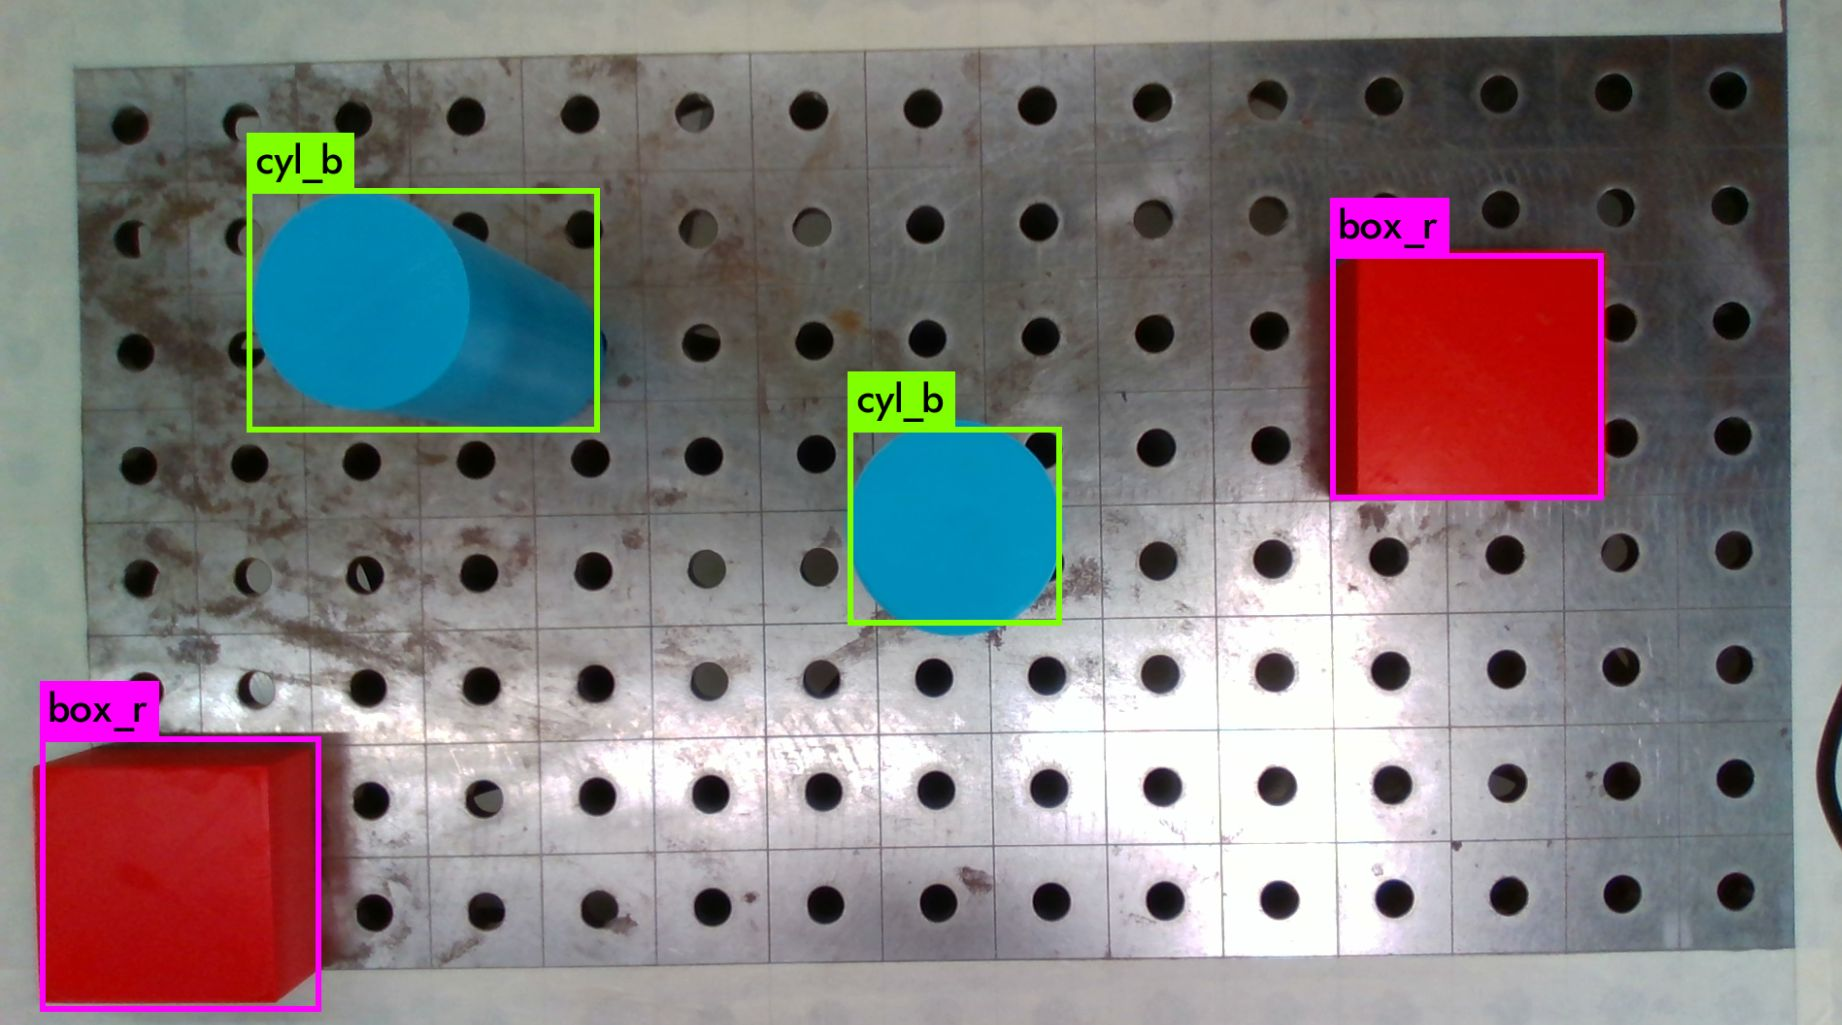
\includegraphics[width=\textwidth]{Bilder/rv6l_boxes.jpg}
    \caption{rv6l\_3d Bounding Boxes}
    \label{fig:rv6l_boxes}
\end{figure}

\newpage
Die Rückgabe des \textit{Bounding Box Publishers} ist im Paket folgendermaßen umgesetzt \seeAtt{sec:rv6l_3d} [C++]:

\begin{lstlisting}[language=c++]
[ . . . ]
        midx = (maxx + minx) / 2; // Objektmittelpunkt (x)
        midy = (maxy + miny) / 2; // Objektmittelpunkt (y)
        midz = (maxz + minz) / 2; // Objektmittelpunkt (z)
      }
    
    rv6l_3d_msgs::RV6L_position bbx_msg;
    bbx_msg.Class = bbx.Class;              // Klasse
    bbx_msg.probability = bbx.probability;  // Wahrscheinlichkeit

    bbx_msg.w = midy; // "horizontale" Position im Bild
    bbx_msg.h = midz; // "vertikale" Position im Bild
    bbx_msg.d = minx; // Abstand (min) durch Point Cloud

    boxes->bounding_boxes.push_back(bbx_msg); // Rueckgabe an BB Message
[ . . . ]
\end{lstlisting}

Die modifizierte \textit{Message} des \textit{rv6l\_3d}-Pakets setzt sich somit aus diesen Werten zusammen:

\begin{lstlisting}[language=python]
string Class         # Objektklasse
float32 probability  # Confidence
float32 w            # horizontale Koordinate im Bild (width)
float32 h            # vertikale Koordinate im Bild (height)
float32 d            # Abstand zum Objektmittelpunkt (depth)
\end{lstlisting}

Es werden Objektklasse, Erkennungssicherheit und die Mittelpunktkoordinaten ausgegeben. Der Datentyp \textit{float32} wird von \textit{C++} und \textit{Python} als \textit{float} interpretiert, weshalb er sich gut für die Übermittlung eignet. Die Koordinaten der Objekte werden relativ zum Kameramittelpunkt unter Berücksichtigung des Abstands zum Objekt in Metern ausgegeben. Dabei ist $w$ in Richtung Bildoberseite und $h$ in Richtung der rechten Bildkante positiv. Der Abstand $d$ beginnt mit $0$ an der Kameraoberfläche und kann nur positive Werte annehmen.
Bei der Abstandsberechnung wird der Abstand zwischen der $h$-$w$-Ebene der Kamera \seeFig{fig:realsense_koord} und der $x$-$y$-Ebene des Basiskoordinatensystems genutzt, sodass dieser unabhängig vom horizontalen Versatz zwischen Objekt und Kamerasystem immer die gleiche Distanz zurückgibt.

\begin{figure}[ht]
    \centering
    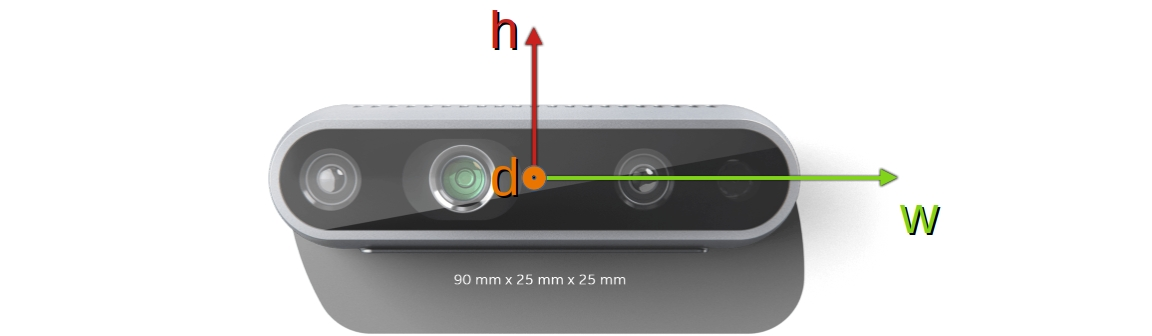
\includegraphics[width=\textwidth]{Bilder/realsense_koord.jpg}
    \caption{Koordinatensystem der Intel RealSense, Abbildung nach \cite{intel_corporation_depth_2022}}
    \label{fig:realsense_koord}
\end{figure}

Das Programm gibt die ermittelten Positionen in Form eines \textit{Topics} an den \textit{Subscriber} des Programms für die Bewegungssteuerung des Roboters weiter:

\subsection{Bounding Box Subscriber}

Der \textit{Subscriber} nimmt die vom \textit{rv6l\_3d} ermittelten Rückgabewerte auf und speichert diese in einer Liste \seeAtt{sec:handhabung} [Python]:

\begin{lstlisting}[language=python]
[ . . . ]
        def callback_pos(self, data):
            for box in data.bounding_boxes:
                self.object_pos_cam = [box.Class, box.h, box.w, box.d]
[ . . . ]
\end{lstlisting}

Diese Liste kann dann vom Bewegungssteuerungsprogramm (basierend auf Steinbeck \cite[Abschnitt~3.5.2]{steinbeck_entwicklung_2022}) zum Anfahren der Zielpositionen genutzt werden. Dieser Algorithmus wurde zur Nutzung mit der Objekterkennung folgendermaßen angepasst:

\subsection{Algorithmus zur Positionserkennung} \label{subsec:algorithmus_positionserkennung}

Für die Positionserkennung müssen die Koordinaten des Objekts in Relation zum Basiskoordinatensystem bekannt sein:
\begin{equation*}
    \tensor[^{G}]{\mathrm{\underline{p}}}{} (G \to Cam) = \tensor[^{G}]{\mathrm{\underline{p}}}{} (G \to Tool) + \tensor[^{G}]{\mathrm{\underline{p}}}{} (Tool \to Cam) 
\end{equation*}

Die aktuelle Transformation vom in \refFig{fig:rv6l_basis} eingezeichneten Koordinatensystem $G$ in das Kamerakoordinatensystem $Tool$ $\tensor[^{G}]{\mathrm{\underline{p}}}{} (G \to Tool)$ kann jederzeit ausgelesen werden. Somit muss für die Bauteilpositionsbestimmung die Transformation $\tensor[^{G}]{\mathrm{\underline{p}}}{} (Tool \to Cam)$ durchgeführt werden. 

\begin{figure}[ht]
    \centering
    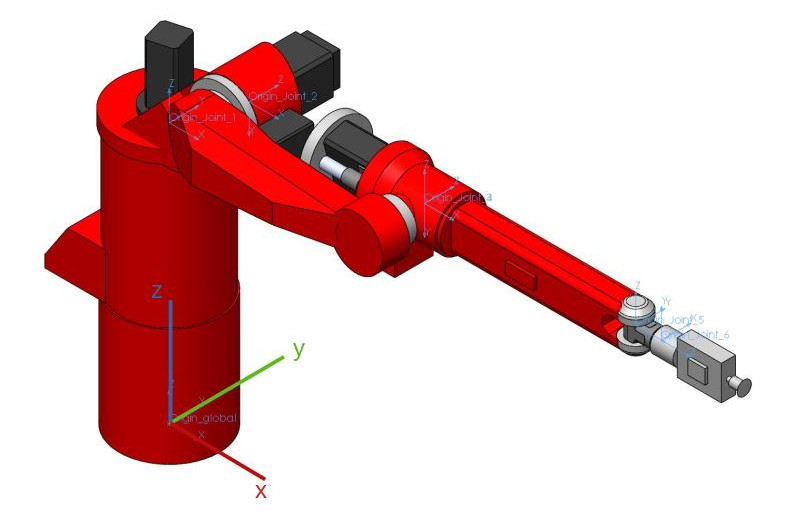
\includegraphics[width=9cm]{Bilder/rv6l_basis.jpg}
    \caption{Koordinatensystem des RV6L, Abbildung nach \cite[Abbildung~12]{leber_steuerung_2021}}
    \label{fig:rv6l_basis}
\end{figure}

Die Tabelle in \refFig{fig:realsense_transformation} zeigt eine Tabelle zur Umrechnung der Orientierungen aller Koordinatensytsteme. Diese gilt ausschließlich für die im Test verwendete Orientierung mit einer Drehung von $90$° gegenüber dem Endeffektor und einer Ausrichtung des Endeffektors parallel zur $x$-Achse und zur $x$-$y$-Ebene \seeFig{fig:realsense_halter}. Dabei ändert sich die Orientierung im Schritt der Bilderkennung des verwendeten Algorithmus nicht, weshalb nur die Translation berechnet werden muss. Diese wird hier als Kameraoffset bezeichnet:

\begin{align*}
    x_{pCam} & = x_{pTool}+o_{x}\\
    x_{pObj} & = x_{pCam}+h_{pObj}\\
    x_{pObj} & = x_{pTool}+o_{x}+h_{pObj}\\\\
    y_{pCam} & = y_{pTool}+o_{y}\\
    y_{pObj} & = y_{pCam}+w_{pObj}\\
    y_{pObj} & = y_{pTool}+o_{y}+w_{pObj}\\\\
    z_{pCam} & = z_{pTool}-o_{z}\\
    z_{pObj} & = z_{pCam}-d_{pObj}\\
    z_{pObj} & = z_{pTool}-o_{z}-d_{pObj}
\end{align*}

Alle Variablen stehen in Bezug zum Koordinatensystem $G$. $[...]_{pCam}$ beschreibt die Position der Kamera, $[...]_{pTool}$ die des Tool-Koordinatensystems und $[...]_{pObj}$ des Objekts. $o_{[...]}$ ist der Offset zwischen Kamera und Tool. 

\begin{figure}[ht]
    \centering
    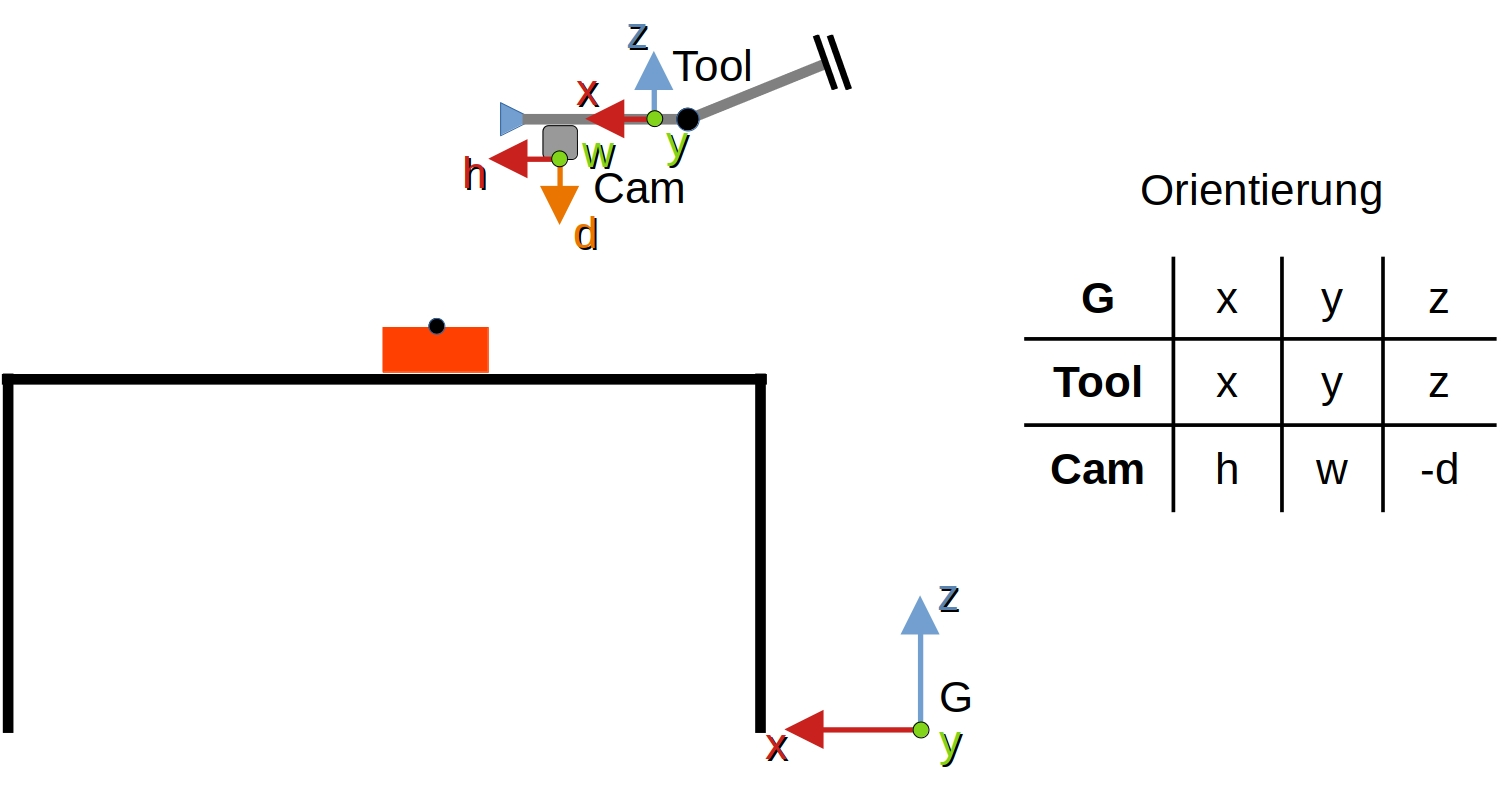
\includegraphics[width=\textwidth]{Bilder/realsense_transformation.jpg}
    \caption{Objektkoordinaten}
    \label{fig:realsense_transformation}
\end{figure}

Die Positionserkennung ist folgendermaßen implementiert [Python]: \footnote[3]{Basiert auf \cite{steinbeck_entwicklung_2022}, \seeAtt{sec:handhabung}. Unwichtige Funktionsaufrufe und -definitionen wurden zur Verbesserung der Übersichtlichkeit entfernt}

\begin{lstlisting}[language=python] 
STATIC_X = 0.237  # Offset in X-Richtung (Greifposition)
STATIC_Y = 0      # Offset in Y-Richtung (Greifposition)
STATIC_Z = 0.237  # Offset in Z-Richtung (Greifposition) = STATIC_X durch Orientierungswechsel
    
SCAN_NEAR = 0.30  # Hoehe fuer nahen Scan
        
[ . . . ]

    py.go_to_scan_pose()  # Scanposition anfahren
    
    ichbinder = uwe() # Klasse aus subscriber_cam initialisieren, Objektpos. auslesen
    rospy.wait_for_message("/darknet_ros_3d/bounding_boxes/", RV6L_positions, timeout=None) # Warten auf Nachricht mit Objektposition relativ zur Kamera
    cam_pos = ichbinder.object_pos_cam  # Aktuelle Position in cam_pos speichern
                         
    py.go_to_scan((cam_pos[1] + REF_X), (cam_pos[2] + REF_Y),(REF_Z - cam_pos[3] + SCAN_NEAR))  # Anfahren der Scanposition ~ ueber dem Bauteil
    
    cam_near = ichbinder.object_pos_cam # Ermitteln des genauen Objektmittelpunktes
        
    py.go_to_pose_goal((cam_pos[1] + REF_X + cam_near[1] + STATIC_X), (cam_pos[2] + REF_Y + cam_near[2] + STATIC_Y), (REF_Z - cam_pos[3] + STATIC_Z - (cam_near[3] - SCAN_NEAR) + 0.25)) # Greifposition anfahren
    
    py.go_to_pose_goal((cam_pos[1] + REF_X + cam_near[1] + STATIC_X), (cam_pos[2] + REF_Y + cam_near[2] + STATIC_Y), (REF_Z - cam_pos[3] + STATIC_Z - (cam_near[3] - SCAN_NEAR))) # Endeffektor absenken
\end{lstlisting}

Der Roboter fährt zuerst in eine Position, die den für die Erkennung nutzbaren Gesamtbereich im Kamerabild sichtbar macht (Zeile 9). Anschließend wird ein Scan durchgeführt und die Objektposition in der Variable \lstinline{cam_pos} gespeichert (Zeile 13). Diese Position ist im Kamerakoordinatensystem \seeFig{fig:realsense_koord} angegeben. Aufgrund der Perspektive und der Funktionsweise der \textit{Bounding Boxes} weicht der Mittelpunkt jedoch vom realen Bauteilmittelpunkt ab. Diese Abweichung ist in \refFig{fig:rv6l_boxes} erkennbar.

Wegen der Abweichung wird diese ungefähre Mittelpunktposition mit dem Mittelpunkt der Kamera in der $x$-$y$-Ebene $30cm$ über dem Bauteil angefahren. Dadurch ist nur noch die Objektoberseite sichtbar, sodass der genaue Objektmittelpunkt bestimmt werden kann (Zeile 15). Zum Ermitteln der Zielkoordinaten werden die Startkoordinaten und die von der Kamera ermittelten Objektkoordinaten gemäß der in \refFig{fig:realsense_transformation} dargestellten Umrechnungstabelle addiert. Außerdem werden $30cm$ (Variable \lstinline{SCAN_NEAR}) zum Anfahren der korrekten Höhe zur $z$-Koordinate addiert. Der Kameraversatz ist in diesem Fall irrelevant, da er in Start- und Zielposition den gleichen Wert hat und somit eliminiert wird. Somit bewegt sich die am Endeffektor befestigte Kamera beim Aufruf der Funktion \lstinline{go_to_scan} zum ungefähren Objektmittelpunkt. Nach Anfahren dieser Koordinaten wird der Mittelpunkt des Objekts erneut ermittelt und in der Variable \lstinline{cam_near} gespeichert (Zeile 17). Dazu wird das Kamerakoordinatensystem verwendet, wodurch nur die Abweichung zwischen Kamera- und Bauteilmittelpunkt gespeichert wird.

Zum Greifen des Bauteils muss der Versatz und die Rotation zwischen Kamera und Endeffektor beachtet werden. Die Variablen \lstinline{STATIC_<...>} legen diesen Offset zwischen Kamera und $Tool$-Koordinatensystem fest. Sie unterscheiden sich je nach Roboterkinematik und Kameraposition. Im Test wurde die Intel RealSense mit einem Offset von $23,7cm$ in $x$-Richtung und $-5,7cm$ zur Vorderkante der Kamera in $z$-Richtung des $Tool$-Koordinatensystems montiert. Somit wird mit \lstinline{STATIC_X} die $x$-Koordinate der anzufahrenden Position um $23,7cm$ erhöht, damit das $Tool$-Koordinatensystem in der Greifposition sich mit der $x$-Koordinate der Kamera in der Scanposition deckt. Im vorliegenden Fall ist aufgrund des Orientierungswechsels zwischen Scan- und Greifposition der Versatz zwischen Kamera und $Tool$ von $23,7cm$ in $x$-Richtung äquivalent zum Versatz der Scanposition in $z$-Richtung \seeFig{fig:rv6l_positionen}. Der Kameraoffset kann beispielsweise durch Messungen am realen System ermittelt werden. Im angefügten Quellcode wurde der Wert \lstinline{STATIC_Z} durch experimentelle Annäherung leicht angepasst.

\begin{figure}[ht]
    \centering
    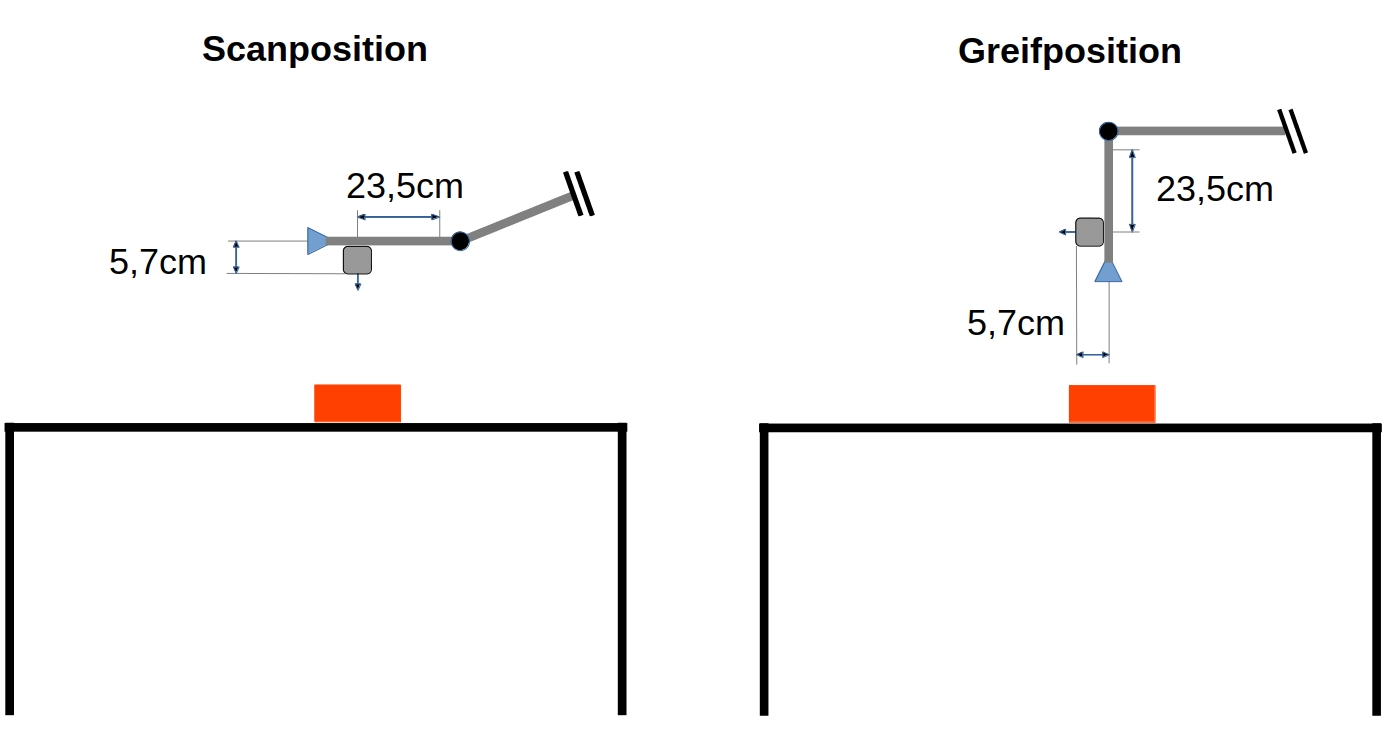
\includegraphics[width=\textwidth]{Bilder/rv6l_positionen.jpg}
    \caption{Roboterpositionen}
    \label{fig:rv6l_positionen}
\end{figure}

Im nächsten Schritt wird die Funktion \lstinline{go_to_pose_goal} aufgerufen (Zeile 19). Diese fährt die Zielposition im Gegensatz zur \lstinline{go_to_scan}-Funktion nicht in \mbox{Scan-,} sondern in Greifposition an. Somit erfolgt hier der erwähnte Orientierungswechsel. Als Zielkoordinaten werden hier sowohl die in \lstinline{cam_near} gespeicherten genauen Offset-Werte für den Bauteilmittelpunkt, die anzufahrende Höhe von $25cm$ vor Absenken des Endeffektors, als auch die Werte der \lstinline{STATIC_[...]}-Variablen zu den anfangs ermittelten Koordinaten addiert, wodurch die genaue Zielposition angefahren wird. Im letzten Schritt wird der Greifer um die erwähnten $25cm$ abgesenkt, um das Bauteil zu greifen.
